%----------------- CHAPTER 5 -------------------------------------------
%--- SERVOS, SERVOS, SERVOS        -------------------------------------
%% Describes the major servo controls and why they are the way they are.
%% 
%% 
%% 
\chapter{The Control Systems}
\label{chap:controls}

\begin{figure}[!h]
\centerline{\includegraphics[angle=0,width=6.5in]{Figures/Chap5/L1LSC.pdf}}
\label{fig:LSCscreen}
\end{figure}
\clearpage

This chapter describes the major feedback control systems used to keep
the interferometer operating at a point of high sensitivity, and
motivations for the requirements on the control loops and their performance
as of 2003.

Most of the assertions made about the signal readout and the noise couplings
in Chapters~\ref{chap:signals}  and \ref{chap:noise}, respectively, are only 
valid at a very specific operating point: the point at which 
the light is resonant in all parts of the interferometer.

Firstly, resonance means that the round trip phase shift in a single cavity is 
an integer multiple of $2 \pi$. This is to ensure that there is constructive
interference and therefore resonant buildup of the field in the cavity.
In the one-dimensional picture where only the distance between the mirrors
may be adjusted, this is a clear definition.

Secondly, the beam must spatially overlap the same region on each pass. If
the cavity mirrors are overly misaligned the beam will simply miss the
mirrors and fall out of the cavity. Between this gross level and perfect
alignment, there will be some reduction in the power buildup. There will
also be some increased noise couplings~\cite{Yaron:Alignment}.

Finally, the beam's wavefront must remain unchanged on each round trip. This
sets some constraint on the shape of the cavity mirrors. In fact, all of
these criteria are just specific examples of a more general criterion which
states that if the electric field is represented in a basis of
orthogonal modes, the
case of perfect resonance is one in which there is no mode mixing on any
round trip of the cavity. This is further described in Appendix~\ref{app:modes}.

The job of the control systems is to keep the light resonating in the
interferometer. Secondarily, the control systems keep the interferometer's
lengths and angles as close as possible to the perfect resonance condition
in order to prevent degradation of the strain sensitivity.

At last count, there were 107 custom tailored, control loops running the 
interferometer; this does not include any of the systems associated with the 
building HVAC controls, the vacuum system, or the several PID type servos
running inside of some of the commercial instruments. At the time of this
writing there are no servos in operation to actively control the mirrors'
curvature. 

This chapter will focus on the active control of the length 
degrees of freedom of the interferometer, with only a brief description of
the angular controls.


\section{The Length Control Loops}
\label{sec:LSC}

The most recent descriptions of the interferometer's length controls are given
in \cite{Sigg:Readout} and \cite{S1:Inst}. The following paragraph gives a
brief description of the generalities. The rest of the chapter goes into more
detail by first motivating the need for control loops and setting requirements
for them. Then constraints are placed on the loops in the gravitational wave band to reduce
noise pollution from the auxiliary loops.

The average arm length is used in the overall frequency stabilization
scheme and is discussed separately in Section~\ref{sec:CMservo}.

There are several common elements among the 4 control loops:

\begin{itemize}
\item An RF photodetector is used to detect the AM modulated light
      exiting from one of the 3 detection ports. The RF signal is
      demodulated at the resonant sideband frequency ($f_{m}$).
      Both the in-phase and the quadrature-phase components of the
      demodulation are acquired by a 16 kHz ADC after a few stages
      of signal conditioning.

\item The signals are all sent to a VME or rackmount CPU, running custom
      written digital signal processing (DSP) code. The code performs
      many functions including: digital filtering, signal summation,
      triggering, and also provides the signals to the  data 
      acquisition system.

\item After some filtering, the digital signals are passed on to
      a separate set of processors which are set up to handle
      all functions of a specific suspended optic. There are
      typically 1 or 2 optics controlled per CPU.

\item These suspension processors then send the final output signals
      for each optic to a digital-to-analog converter (DAC). The
      DAC signals then go through a set of signal conditioning
      circuits. Finally, there is a power amplifier stage for each
      coil of every suspended optic.

\item The coil currents induce forces on the optic through the magnets
      glued onto them. The interferometer lengths and angles are 
      adjusted by moving the suspended optics.
      
\end{itemize}

\begin{figure}[!h]
\centerline{\includegraphics[angle=0,width=6.5in]{Figures/Chap5/LSC.png}}
\caption[LSC Block Diagram]{Block diagram of the Length Sensing and Control
                            system.}
\label{fig:LSCblock}
\end{figure}


\subsection{Allowed Residual Deviations}
\label{sec:residual_req}

The interferometer is said to be 'locked' when the light is resonating
and the error signals of the control loops are still within their linear
region. To determine how tightly the servos must hold the lock one must
look at the stricter constraint of the apparent strain noise
induced by the deviation from perfect resonance.

So for the length degrees of freedoms a requirement is set on either
$\delta L(f)$, the residual error point spectrum or on 
$\delta L_{\mbox {\tiny RMS}}$,
the total RMS deviation.

\subsubsection{Differential Arm Length ($\delta L_-$)}

As shown in Chapter~\ref{chap:noise}, there are a few noise terms which 
scale linearly with $\delta L_-$. Both the laser amplitude noise and the 
oscillator amplitude noise are really the same physical noise mechanism; 
they modulate the gain of the gravity wave readout channel. 
Seen in that light, the requirement is really on the allowed dynamic 
range of the readout signal. Given that the displacement noise goal is 
$1 \times 10^{-19} \, \mbox{m}/\sqrt{\mbox{Hz}}$
at 150 Hz, the requirement must be that the product of the low frequency
error signal and the gain modulation not exceed this level.

Since the noise term is linearly dependent on two variables, the noise
can be decreased by lowering either component. In practice, attempts
were made to suppress both terms. Further iteration was determined by the
success (or lack of it) in these attempts at suppression.

As a rough estimate, we set the requirement for the residual differential
arm length fluctuations to be that 
{\mathversion{bold} $\delta L_- < 1 \times 10^{-13} \, \mbox{m}_{\mbox {\tiny RMS}}$}.
This sets the requirement on the absolute gain modulation to be such that
$\delta G < 10^{-7}$ for $f = 10-10000  \mbox{Hz}$. 
This ensures that the bilinear noise introduced by laser amplitude noise does 
not exceed 1/10 the displacement sensitivity goal. 


\subsubsection{Differential Recycling Cavity Length ($\delta l_-$)}
Excess noise in the sensing of this degree of freedom couples into the
AS port through the $l_{-}$ control loop. The coupling is determined by
Equation~\ref{eq:mich2darm} . Amplitude noise shows up in this loop the same as
for the $L_{-}$ loop. We would like the amplitude noise term
to not exceed the shot limited sensitivity at this port.

From the shot noise formula for MICH in Appendix I, we have that the
shot noise limited sensitivity is 
$1 \times 10^{-16} \, \mbox{m}/\sqrt{\mbox{Hz}}$.
Using the requirement for the gain modulation, we have a requirement
on the residual differential recycling cavity length that
{\mathversion{bold} $\delta l_{-} < 1 \times 10^{-9} \, \mbox{m}_{\mbox {\tiny RMS}}$}.


\subsubsection{Common Arm Length ($\delta L_+$)}

In order to retain the high power buildup in the interferometer, the
coupled cavity formed by the recycling mirror and the arms must stay
quite close to resonance. The field in the recycling cavity, just
past the recycling mirror is
\begin{equation}
E_{RC} = \frac{t_{RM}}{1 + r_{RM} r_{c}} E_{in}
\end{equation}
A small change in the average arm length changes $r_{c}$, the arm
reflectivity, mostly in phase. This moves the carrier off resonance
in the recycling cavity, reducing the overall buildup.

In the limit of perfect contrast, the shot noise at the AS
port is entirely dominated by the sideband power. Then the reduction
in signal-to-noise is proportional to $\sqrt{P_{\mbox{\tiny BS}}}$, the
power on the Beamsplitter, and for
a 1\% reduction in signal-to-noise we can allow a 2\% power reduction.

This sets a limit of 
{\mathversion{bold} $\delta L_{+} < 2 \times 10^{-12} \, \mbox{m}_{\mbox {\tiny RMS}}$}.


\subsubsection{Common Recycling Cavity Length ($\delta l_+$)}

Using the same reasoning as above, the answer for the recycling cavity
common mode length is that 
{\mathversion{bold} $\delta l_{+} < 2.5 \times 10^{-10} \, \mbox{m}_{\mbox {\tiny RMS}}$}.
Here the main difference is that a change in the recycling cavity
length affects the phase of the carrier field in the recycling cavity
directly and does not get the phase gain associated with the arm. In
fact, the ratio between the requirements for the 2 lengths is just the
phase gain factor for the arm, $r_c'$ ($\approx$ 140).

The recycling cavity Finesse for the sidebands is much less than that
for the carrier and as such, the reduction in recycled sideband power
does not drive this requirement.


\subsubsection{External Disturbances}

Ideally one would like to have an accurate model of the interferometer
which could take as inputs all of the available environmental inputs
and deliver all of the interferometer output signals by including
all of the mechanical, electronic, and optical dynamics from one
end of the interferometer to the other. There is currently a time domain
model under development \cite{e2e:Moriond} with exactly this goal.

Even better, however, is to measure the true length fluctuations
interferometrically. So the design of the length control loops is
bootstrapped. The interferometer was first locked with the simplest
loops that would keep it operating in the linear regime. Then the
loop shapes were iterated until the residual fluctuation requirement
was met.

The disturbance, $\Delta(f)$, to a loop can be expressed in terms 
of a few standard servo parameters:

%\begin{align}
%\delta(f) &= \frac{\Delta(f)}{1+G(f)} & C(f) &= \frac{\Delta(f) G(f)}{1+G(f)}
%\end{align}

\begin{equation}
\delta(f) = \frac{\Delta(f)}{1+G(f)}
\end{equation}

\begin{equation}
C(f) = \frac{\Delta(f) G(f)}{1+G(f)}
\end{equation}

From the above equations, one can see that at frequencies where the
open loop gain, $G(f)$, is high, the control signal, $C(f)$, is nearly
equal to the disturbance. At frequencies where the gain is low, the
error signal, $\delta (f)$, is a more accurate estimator. In practice,
to get the most accurate estimate of the disturbance, either the
control signal or the error signal can be used, but both must be corrected
for the transfer function of the servo loop.

Figure~\ref{fig:dist} shows the disturbance signal for the $L_-$, $l_-$, and $l_+$ loops.

\begin{figure}[!h] 
\centerline{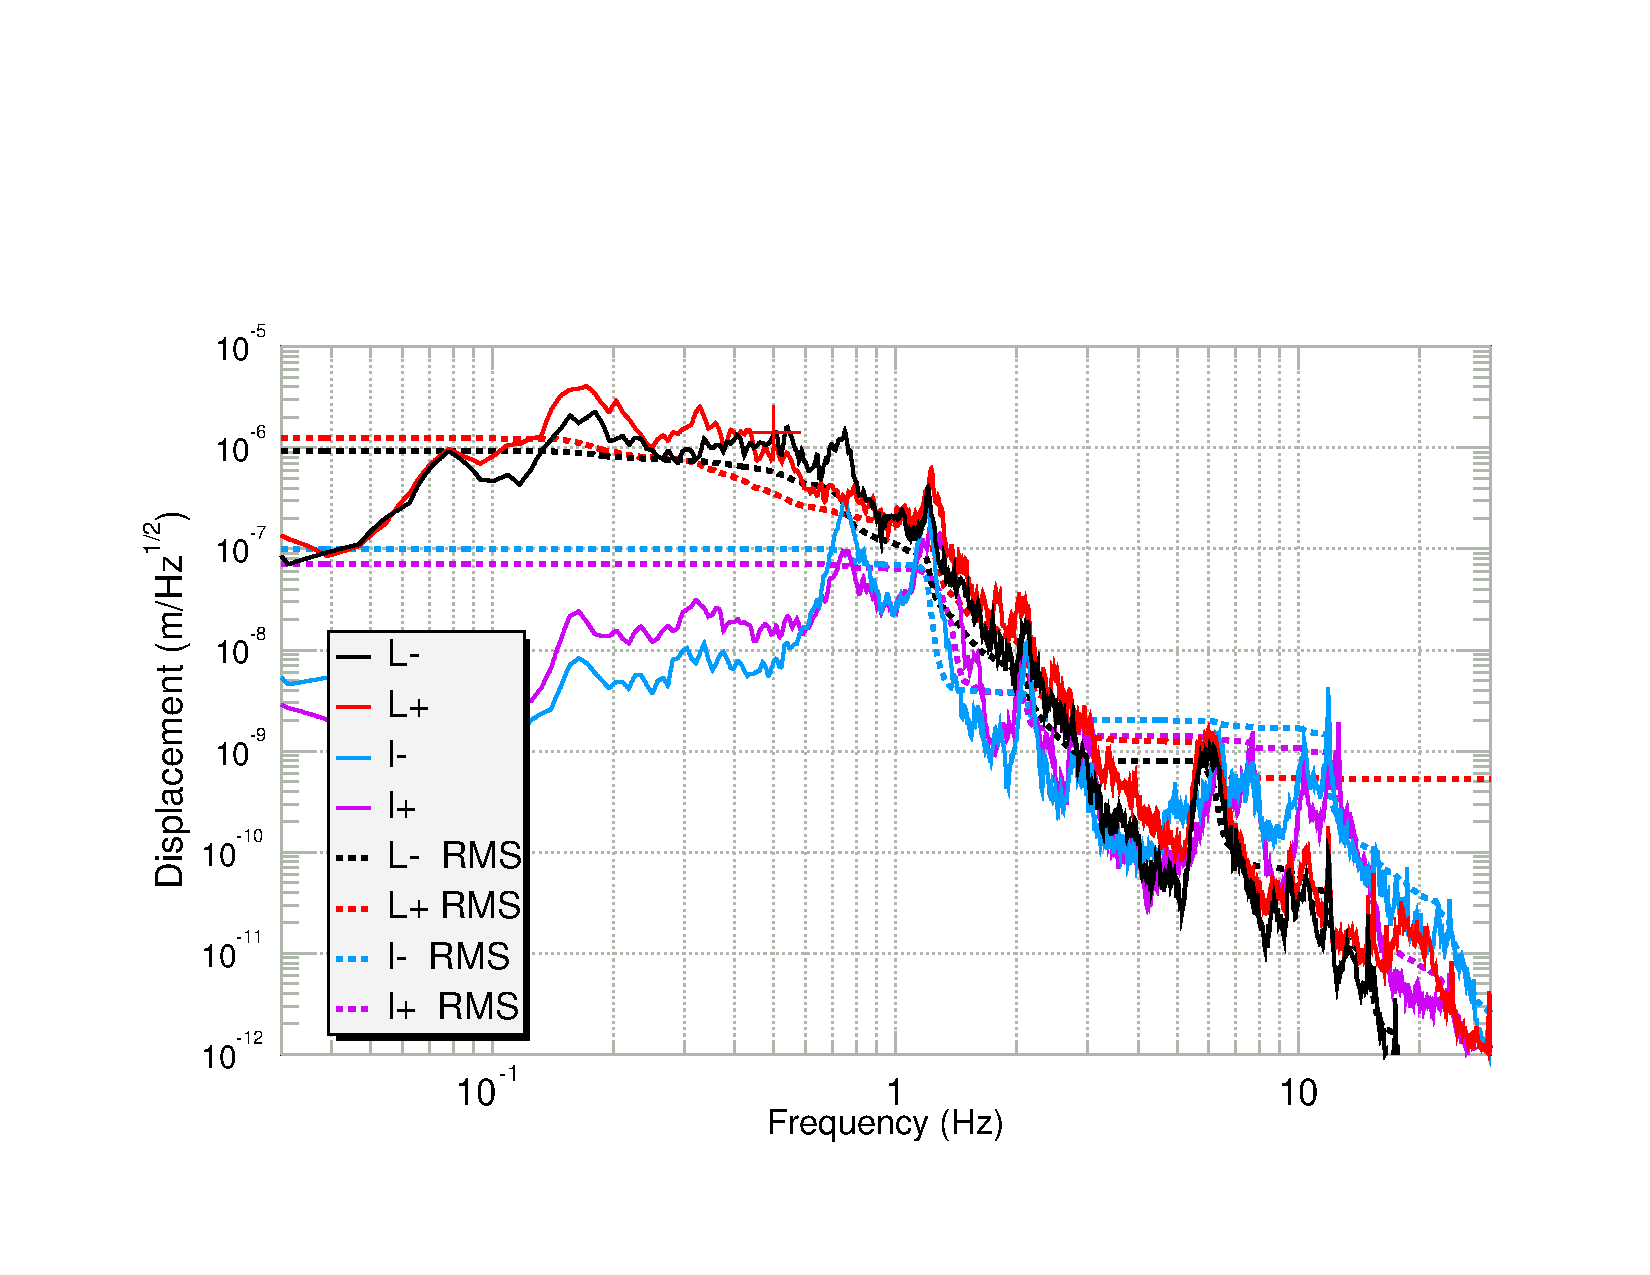
\includegraphics[angle=0,width=6.5in]{Figures/Chap5/disturbances.pdf}}
\caption[Length Disturbances]{Apparent input length disturbance as inferred
         from the servo control signals. The traces labeled 'RMS' show the total
         RMS displacement in the signal in the band,  $f$ - 50 Hz.}
\label{fig:dist}
\end{figure}


\subsubsection{Gain Requirements}

Having the external disturbance spectra and a goal for the residual 
fluctuations allows us to make a first iteration on the control loops. The
fact that the loops are digitally implemented allows one to quickly iterate
on the loop transfer functions and achieve the desired performance.

The Bode plots in Figure~\ref{fig:Loops} show the open loop gain of 
three of the four main length control loops.

\begin{figure}[!h] 
\centerline{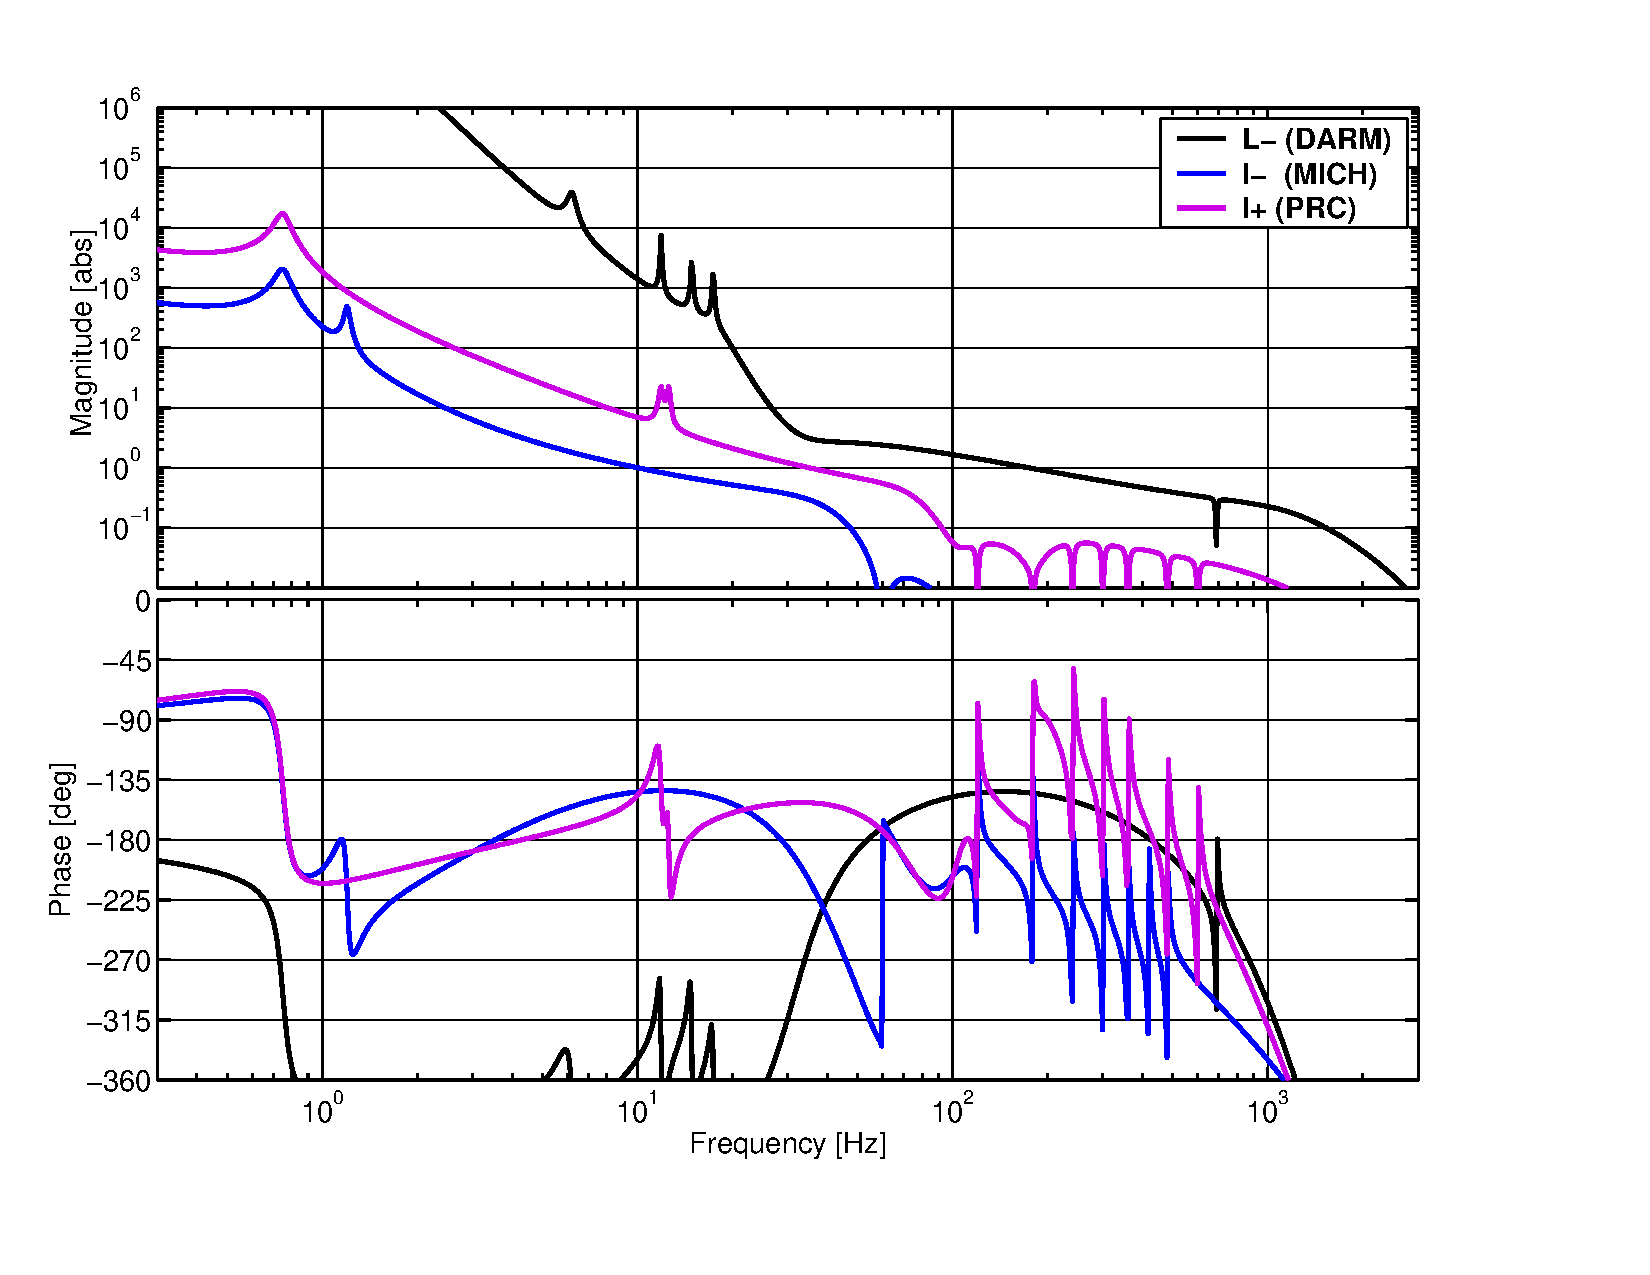
\includegraphics[angle=0,width=6.5in]{Figures/Chap5/LSC-Loops.pdf}}
\caption[Length Loops]{Open loop gain of three length control servos.}
\label{fig:Loops}
\end{figure}
With these loops the measured loop residuals meet the requirement. 
Figure~\ref{fig:residuals} shows the in loop error signals.

\begin{figure}[!h] 
\centerline{\includegraphics[angle=0,width=6.5in]{Figures/Chap5/residuals.png}}
\caption[Residual Fringe Offsets]{Spectra of the servo error points calibrated
         in meters. These are the true length offsets, assuming no significant
         offsets are added in at the error point.}
\label{fig:residuals}
\end{figure}


\subsection{Noise Pollution}

In the gravitational wave band the motion in the auxiliary loops must be controlled to a level
such that induced strain noise spectral density is at the SRD/10 level. The
introduced noise is a function of three parameters of the auxiliary loop:
the sensing noise, the loop gain, and the coupling to AS\_Q. So attempts
were made to reduce all three terms.

\subsubsection{Auxiliary Sensing Noises}

In Figure~\ref{fig:POBnoise}, the noise in the $l_-$ and $l_+$ loops is shown. 
All of the noise above 20 Hz can be seen as some sort of sensing noise in 
that it is not a direct representation of length fluctuations. 

\subsubsection{Gravitational wave band filtering}

Since the $l_{-}$ \& $l_{+}$ signals are full of only sensing noise in
the gravitational wave band one would like to reduce, as much as possible, the contribution
of the control signals to AS\_Q. To do this, aggressive digital stopband
filters were designed to lower the loop gain in the sensitive 60-200 Hz
band.


\subsection{The real loops}

Each of the three main length control loops were individually tailored and
have intricate transfer functions (as shown in Figure~\ref{fig:Loops}).
These following sections list a few of the driving considerations involved
in designing the loops. In all cases, the gain at low frequencies must be
high enough to suppress the noise shown in Figure~\ref{fig:dist} to the
levels specified in Section~\ref{sec:residual_req}. In addition, the servos
must have sufficient gain and phase margin to remain stable in the face
of fluctuating optical gain.


\subsubsection{L$_-$ (a.k.a. DARM)}

The DARM loop controls the differential arm length. The gravitational wave
signal is reconstructed from the error point signal (AS\_Q) of this loop.

This is the highest bandwidth digital servo loop in the interferometer. It
is limited at high frequencies by the phase shifts associated with the
anti-aliasing filters before the ADC and after the DAC (see 
Figure~\ref{fig:DARMmodel}). 

There is also the issue of the high Q ($\sim 10^5$) mechanical
resonance of the suspension wire at the ($\approx$345 Hz) 'violin' frequency;
there is a poorly understood interaction with this resonance which sometimes
requires attenuation through the use of very narrow digital notch filters.
The coupling seems to come and go; the interferometers often run for months
without notches and without any instability.

At even higher frequencies (e.g. 6.6 kHz, 9.3 kHz, and 13 kHz), the servo must have a low 
enough gain to not excite the even higher Q ($10^5 - 10^7$) internal mode 
resonances of the mirrors themselves. These typically have stopbands of 
80-100 dB, widths of a few Hz (to accommodate the temperature dependent 
frequency drift of the modes), and are very near the Nyquist frequency (8192 Hz) 
of the digital system. The modes
with frequencies greater than 8192 Hz are excited through a double aliasing
effect. They are finitely attenuated by the ADC's anti-aliasing filter, but
then still show up in band at 
$f_{aliased} \simeq f_{Nyquist} - (f_{mode} - f_{Nyquist})$. If not filtered
out, this then propagates out through the DAC and is again aliased up to high
frequencies. This completes a loop involving the internal mode which can then
get excited and cause saturation in the sensing electronics. Once a stopband
filter has been tuned for every mode on every driven optic, the modes are
no longer a problem.


\subsubsection{l$_-$ (a.k.a. MICH)}

The MICH loop has a low ($\sim$10 Hz) unity gain frequency. There are two
reasons for this: 

The gain at high frequencies must be kept low to reduce the
the coupling from $l_-$ sensing noise to $L_-$ strain noise. The unity gain
frequency is constrained by the phase lag due to the $\sim$ 50 Hz bandstop filter.

The other constraint is that this loop has a peculiar intermittent coupling to the 
\emph{roll} mode of the recycling mirror. This mode is at $\approx$18 Hz and will
occasionally get excited and grow exponentially if the MICH unity gain
frequency is set to within a few Hz of 18 Hz. It is not understood why this
coupling is unstable.


\subsubsection{l$_+$ (a.k.a. PRC)}

The PRC loop could be run with as high a bandwidth as the DARM loop and has the
same considerations with respect to higher frequency mechanical resonances. The
main constraint on the bandwidth is the noise coupling. So the gain has been
lowered to add aggressive filtering in the 60-200 Hz band. In the long term
the sensing noise in both the $l_+$ and $l_-$ loops will have to be reduced and
the coupling to the anti-symmetric port reduced through the use of off
diagonal length actuation: driving the $L_-$ length by the just the amount
necessary to cancel the measured coupling factor. This technique was
implemented successfully on the Livingston interferometer for the $l_-$ 
servo during the latest Science Run (S3).



\subsection{The Common Mode Servo}
\label{sec:CMservo}
Gravitational radiation can produce both differential and common mode strains
of the arm cavities. We choose to only use the differential mode read out
for gravitational waves because the common mode signal is polluted with a
large level of laser frequency noise.

There is a choice to be made in what to pick as the reference in all of these
length measurements. For the common arm length this amounts to whether the laser
wavelength should be locked to the arms or the arms locked to the laser. Since
we have made such effort to isolate the test masses from external disturbances
the average arm length proves to be a much better reference at audio frequencies
(above 20 Hz).

\begin{figure}[!h]
\centerline{\includegraphics[angle=0,width=6.5in]{Figures/Chap5/FreqNoiseReq.pdf}}
\caption[Laser Frequency Noise]{The spectral density of the free running 
         frequency noise of the MOPA is compared to the SRD/10 requirement 
         based upon an arm cavity reflectivity difference of 0.5\%.}
\label{fig:FreqNoiseReq}
\end{figure}
From Chapter~\ref{chap:noise}, we have the coupling of frequency noise 
into the strain output.
Figure~\ref{fig:FreqNoiseReq} shows that the laser frequency noise must be 
suppressed by a factor of 10$^8$ to bring it to 1/10th of the strain 
sensitivity goal. There is more to
the problem than just gain, however. As the laser is further quieted, each
following reference to which the frequency is servoed must be more quiet than
the last.

To achieve the required suppression, multiple, hierarchical servos are used.
Before the light is injected into the vacuum, the large, raw laser fluctuations 
are actively and passively suppressed (see Section~\ref{sec:PSL}). 
Laser noise above 1 MHz
is filtered out by passing through a medium finesse ring cavity called
the pre-mode cleaner. By locking the laser frequency to a short ($\approx 20 cm$), 
rigid reference cavity with a $\sim$100 kHz servo loop the laser frequency noise
is stabilized by a factor of $\sim$1000.
 
This pre-stabilized light is then locked to a much quieter, suspended,
12 m cavity called the Mode Cleaner, described in Appendix~\ref{app:ModeCleaner}. 
Finally, the light transmitted through the Mode Cleaner is locked to the 
average length of the 4 km arm cavities.

\begin{figure}[!h]
\centerline{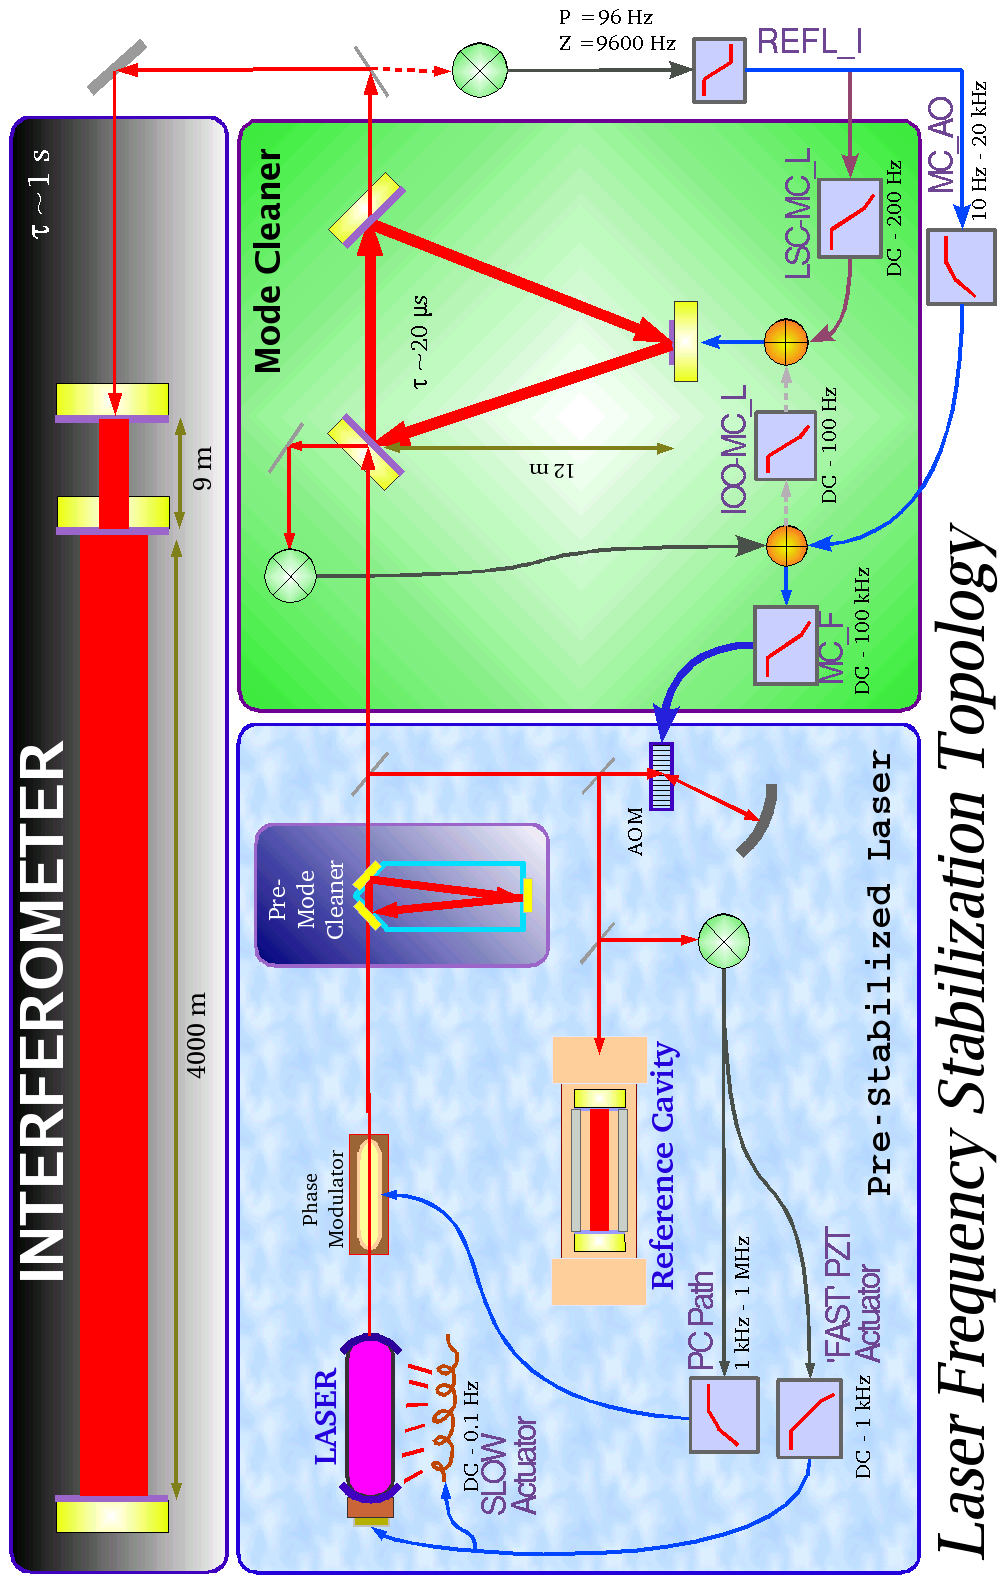
\includegraphics[angle=0,height=7.5in]{Figures/Chap5/CMs90.png}}
\caption[CM Servo Block Diagram]
        {Block diagram of the Global Frequency Stabilization Topology.}
\label{fig:CMblock}
\end{figure}
Ignoring for the moment the internal workings of the mode cleaner and the laser
we can focus on the mechanics of the common mode servo. The difficulty is that
although the laser wavelength is already tightly locked to the mode cleaner
length, it is necessary to adjust the wavelength to match the common mode arm
length and yet keep the light resonating in all the cavities simultaneously.

To see how this is done, it is useful to look at what the MC servo really does.
It derives an error signal which is nominally proportional to the difference
between the round trip length of the cavity and the wavelength of the light
incident on the cavity, modulo an integer number of wavelengths. The common
mode servo works by adjusting the reference to which the laser wavelength
is compared.

At low frequencies, the common mode servo drives the mode cleaner length. This
adjusts the laser frequency since the laser frequency is already locked to the
MC length. Above a few hundred Hz, the length feedback is limited by the
wire resonances of the MC suspension.

A fast, low dynamic-range path, called the additive offset (AO), is used up to 20 kHz.
The AO path works by adding electronic offsets into the MC error
point. The MC servo shifts the laser frequency in order to cancel this offset,
but the resulting laser frequency offset serves the purpose of the AO. 
This might pose a problem, since by introducing an offset in the MC
error point, the laser is being pulled off of resonance in the MC. However,
the actual AO control signal is quite small; only a few Hz peak-peak, as 
compared to the $\sim$8 kHz linewidth of the MC resonance.


\begin{figure}[!h]
\centerline{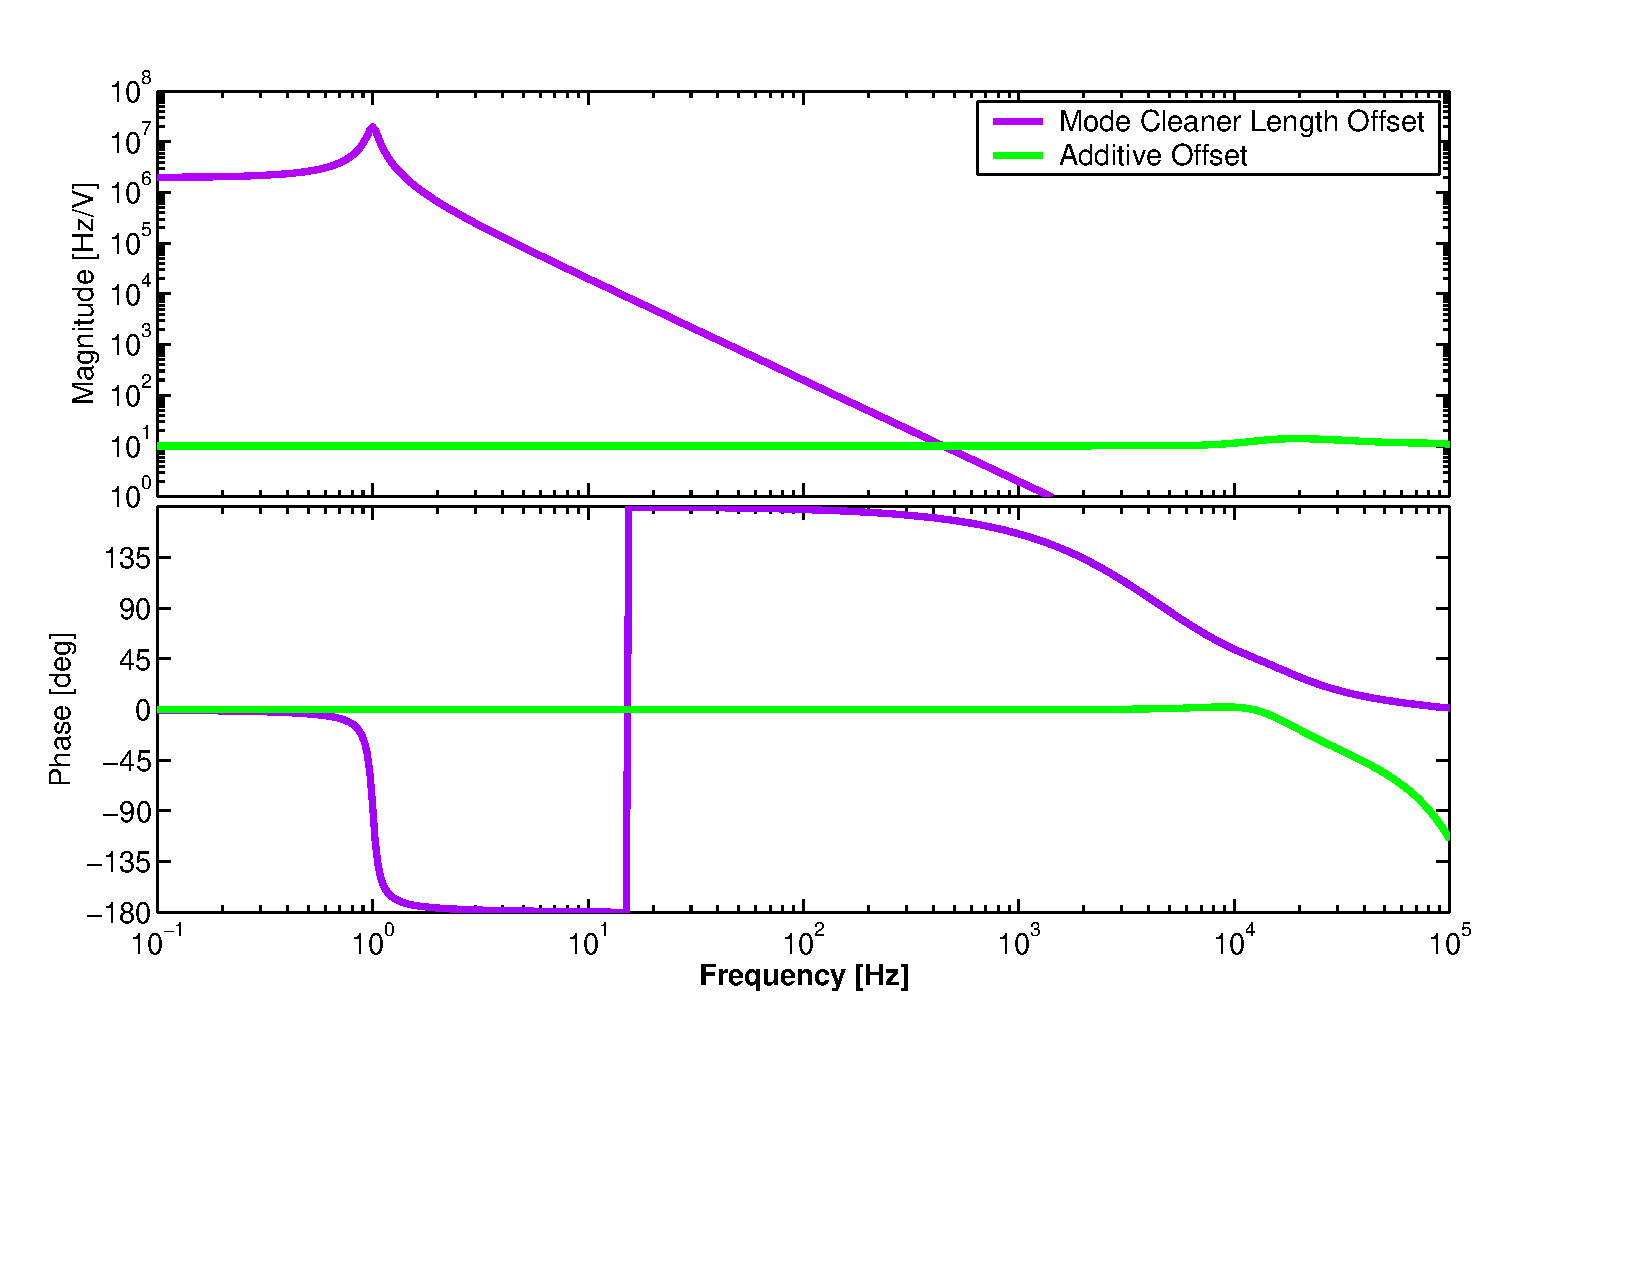
\includegraphics[angle=0,width=6.5in]{Figures/Chap5/cm_acts.pdf}}
\caption[CM Actuators]{Shown are the frequency responses of the two actuators
                       used in the common mode servo. The response is to voltage
                       applied at the coil driver (MCL) and the MC servo mixer
                       (AO).}
\label{fig:CMactuators}
\end{figure}


Figure~\ref{fig:CMactuators} shows the frequency response of the two CM servo
paths. At high frequencies, very large voltages would be required to get
sufficient actuation authority in the MC length path and so the two paths
are crossed over as shown in Figure~\ref{fig:CMbode}. The AO bandwidth is
limited at high frequencies by the finite bandwidth of the MC servo.


\begin{figure}[!h]
\centerline{\includegraphics[angle=0,width=6.5in]{Figures/Chap5/CM-Loops.png}}
\caption[CM Loops]{Open Loop Gain of the total Common Mode Servo and of the
                   individual MCL and AO paths.}
\label{fig:CMbode}
\end{figure}


Figure~\ref{fig:CMcontrols} shows the control signals of the CM servo. In the
regime where the loop gain is high the control signal can be used to estimate
the input disturbance - the frequency noise on the light transmitted by the
MC.


\begin{figure}[!h]
\centerline{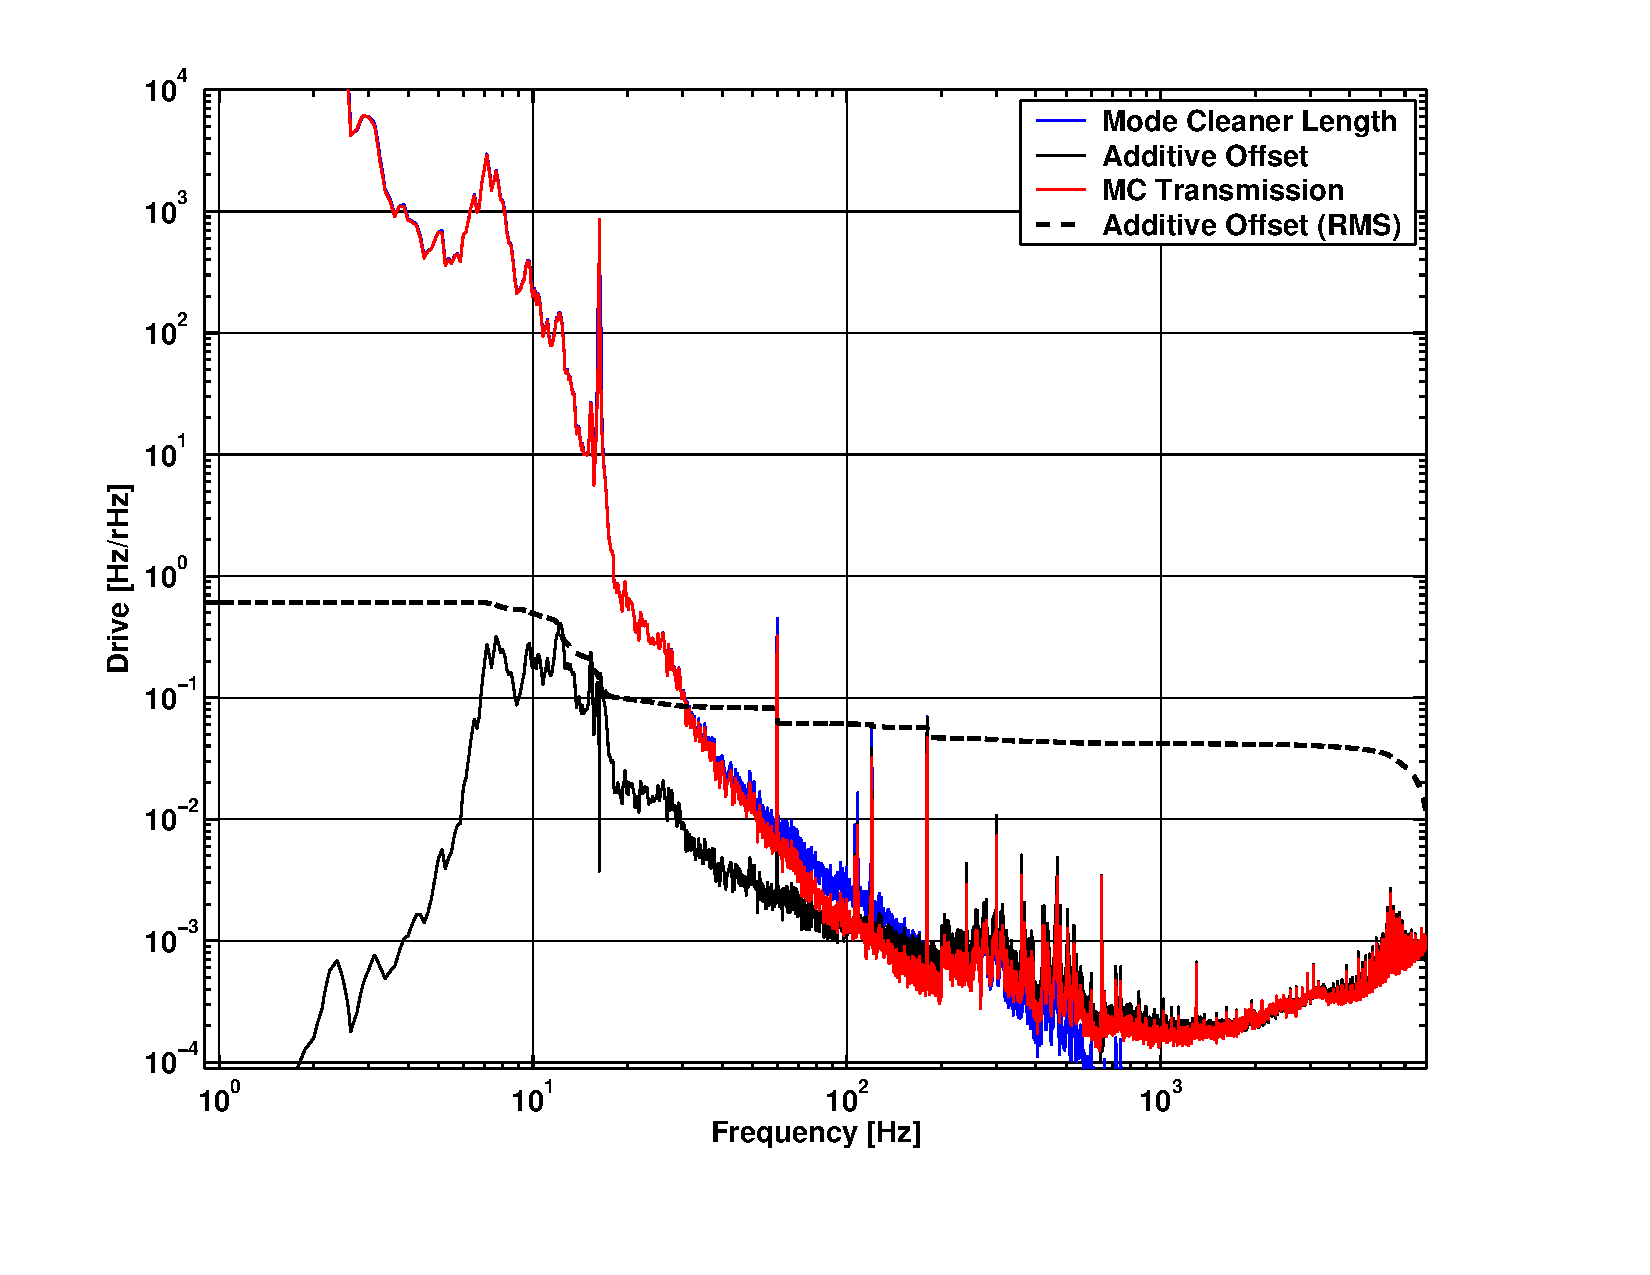
\includegraphics[angle=0,width=6.5in]{Figures/Chap5/cmnoise3.pdf}}
\caption[CM Noise]{The MCL and AO control signals are shown. Also shown is the
         total frequency noise transmitted by the MC, calculated from the CM
         control signals. Also shows is the integrated RMS of the AO control.}
\label{fig:CMcontrols}
\end{figure}


Finally, the ultimate performance of the entire frequency stabilization scheme
can be summed up by Figure~\ref{fig:CMnoise}. The plotted requirement is the
level of frequency noise which will equal 1/10 of the strain sensitivity goal.

This curve is calculated using the frequency domain interferometer model which
uses as inputs the measured frequency noise to differential strain coupling. This
curve along with the measured CM servo loop gain establishes a requirement on the
frequency fluctuations on the light leaving the mode cleaner. This requirement is
compared to the measured performance of the mode cleaner in 
Appendix~\ref{app:ModeCleaner}.

\begin{figure}[!h]
\centerline{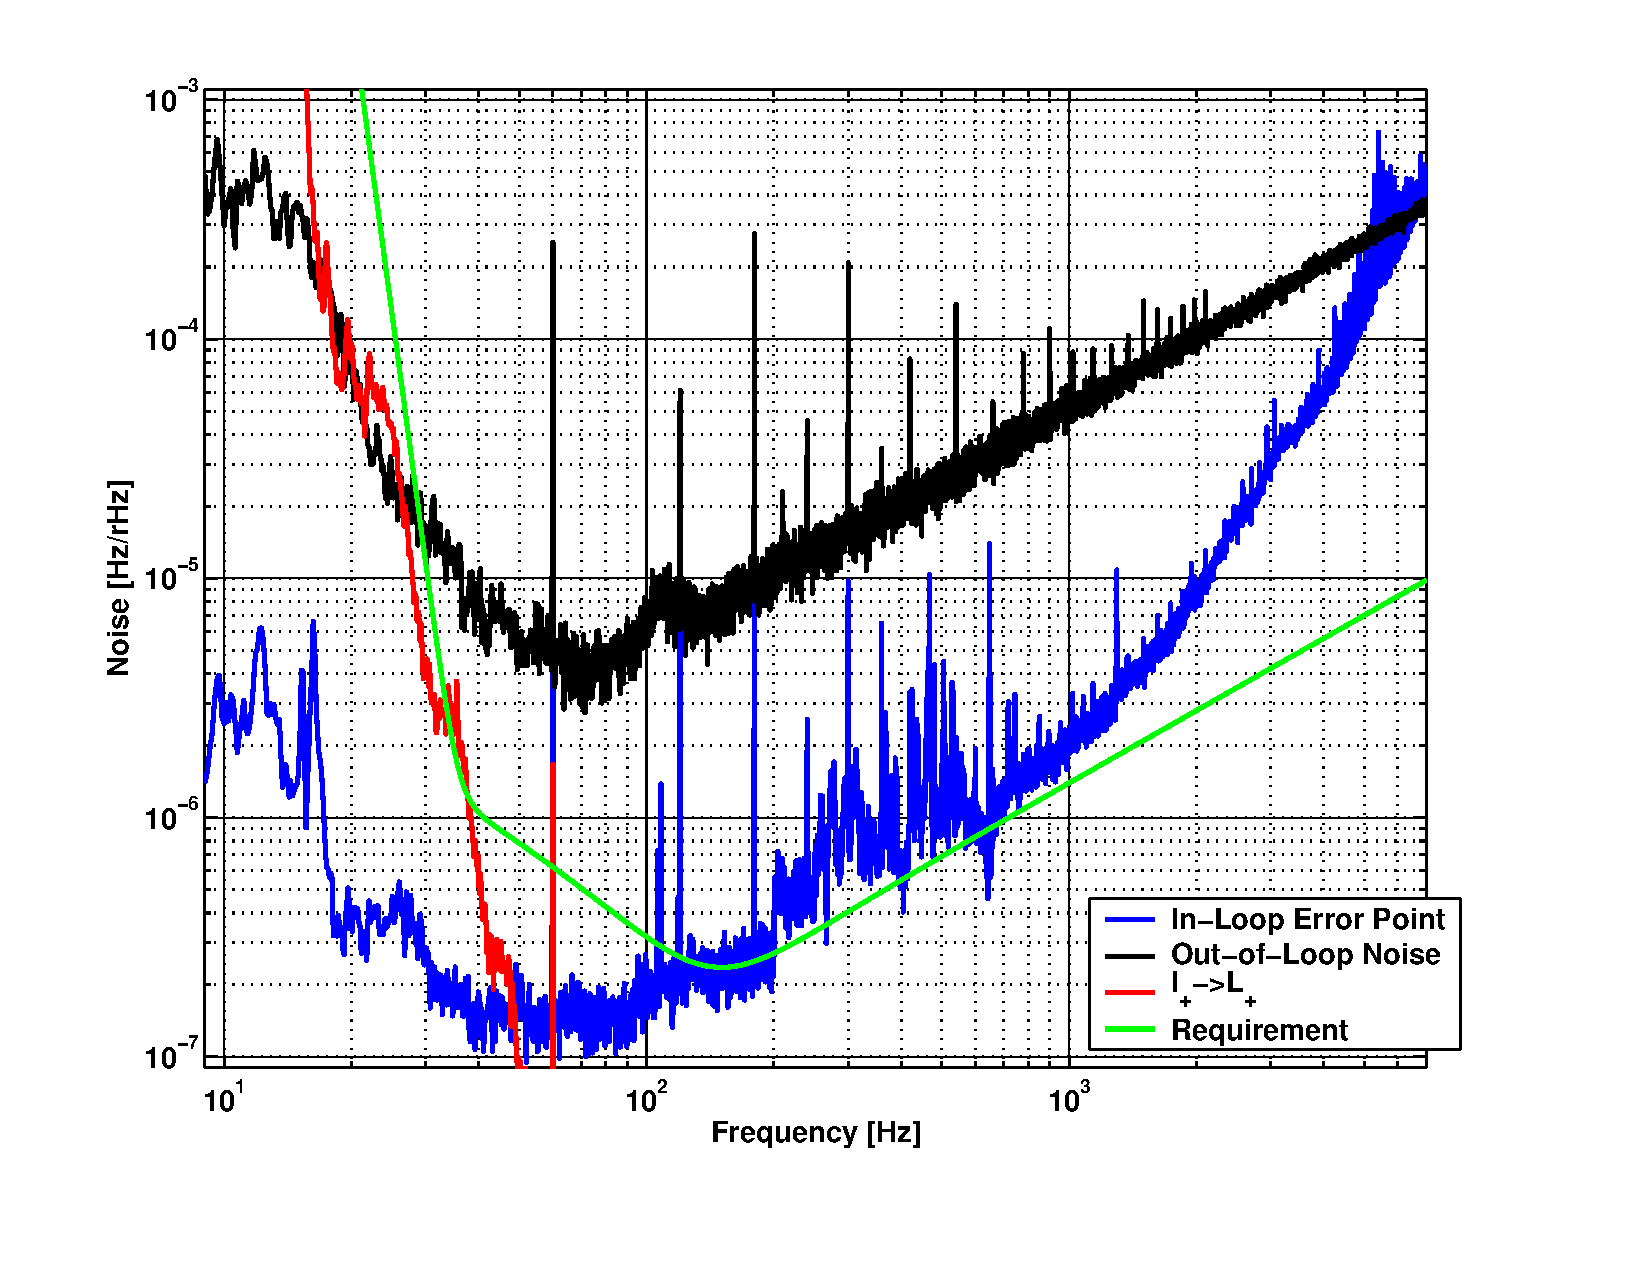
\includegraphics[angle=0,width=6.5in]{Figures/Chap5/cmnoise3b.pdf}}
\caption[Residual Frequency Noise]{The in-loop error point is compared to the
           sensing noise floor to show that the in-loop error point 
           underestimates the true noise. The plotted requirement is SRD/10.}
\label{fig:CMnoise}
\end{figure}

\subsubsection{Parasitic Interferometers}
\label{sec:CMscatter}

On the laser table, vibrations of the optical mounts put phase noise on the light
which then is measured in the mode cleaner control signal. This frequency noise
has been reduced somewhat through the use of stiffer mounts and acoustic isolation
of the table. The mode cleaner servo gain is sufficient to make acoustics from the
laser table an insignificant contributor to the interferometer noise.

Acoustic coupling on the mode cleaner's output optical table dominates the
frequency noise on the light incident on the interferometer in the 100-1000 Hz
band. This still needs to be reduced by $\sim$10.

The acoustic noise on the mode cleaner table is injected at the error point
of the servo as sensing noise. It is only characterized because we then measure the
mode cleaner noise performance with an even quieter reference in the common mode
servo. For the common mode servo, there is no further check and so the acoustic
noise coupling there is sent unsuppressed into the interferometer and is
probably more severe.

The steep rise below 100 Hz in the 'out-of-loop' trace of Figure~\ref{fig:CMnoise} is due
to a parasitic scattering path somewhere in the path between the recycling
mirror and the readout PD for the interferometer's reflected port.


\section{Angular Controls}
\label{sec:ASC}

The Angular Sensing and Control system is still being commissioned and
refined. This section briefly mentions the different angular sensing
schemes which are used. 


There are three chief feedback paths for the angular degrees of freedom
of the interferometer:

\begin{itemize}

\item The first, primitive stabilization is done by damping the pitch
      and yaw eigenmodes of the suspended optics using the local 
      sensors~\ref{sec:OSEMs}. These provide some stability at the
      pendulum frequencies, but is limited by the large motions of the
      isolation stack to which the suspension cage is mounted. The high
      frequency angular sensing noise of the local sensors is
      $\approx10^{-10} \, \mbox{radians}/\sqrt{\mbox{Hz}}$. This requires
      a very low bandwidth servo ($\approx 2$ Hz) with aggressive low
      pass filtering.

\item The second level of angular stabilization comes from optical levers.
      Each optical lever is a fiber coupled diode laser and a
      quadrant photodetector, each mounted to a steel pier outside
      of the vacuum. From $\approx$0.3-5 Hz, these are better angular
      references than the local sensors. Their chief benefit is in simplicity:
      these servos work independent of the locked state of the interferometer.
      The noise in this sensor is somewhat better than the local sensors,
      $\approx10^{-11} \, \mbox{radians}/\sqrt{\mbox{Hz}}$, in a broadband
      sense but is dominated by acoustic/mechanical resonances which
      are 10-50X larger.

\item The ultimate solution to angular sensing is the Wavefront Sensor (WFS)
      system~\cite{Yaron:Alignment,Alignment:Applied,Nergis:Thesis}. These are 
      RF quadrant detectors working
      on a heterodyne readout system similar to that used in the length
      sensing. The WFSs sense relative tilts and translations between the carrier
      and RF sideband fields by taking differences between the demodulated outputs
      of the quadrants. The shot noise limited sensing noise of these sensors
      is, in principle, far superior to the other sensors. The broadband
      noise floor varies from $10^{-13} - 10^{-14} \, \mbox{radians}/\sqrt{\mbox{Hz}}$,
      depending on which sensor.

\item A non-RF part of the WFS scheme is the DC quadrant photodetectors 
      monitoring the weak beams transmitted through the arm cavity end 
      mirrors. These fix the beam position onto the center of the end mirrors.
      The angular sensitivity of these sensors is comparable to the WFS, but
      they have the disadvantage of being fixed to the local reference frame
      of the ground at the end stations.

\end{itemize}


\begin{figure}[!h]
\centerline{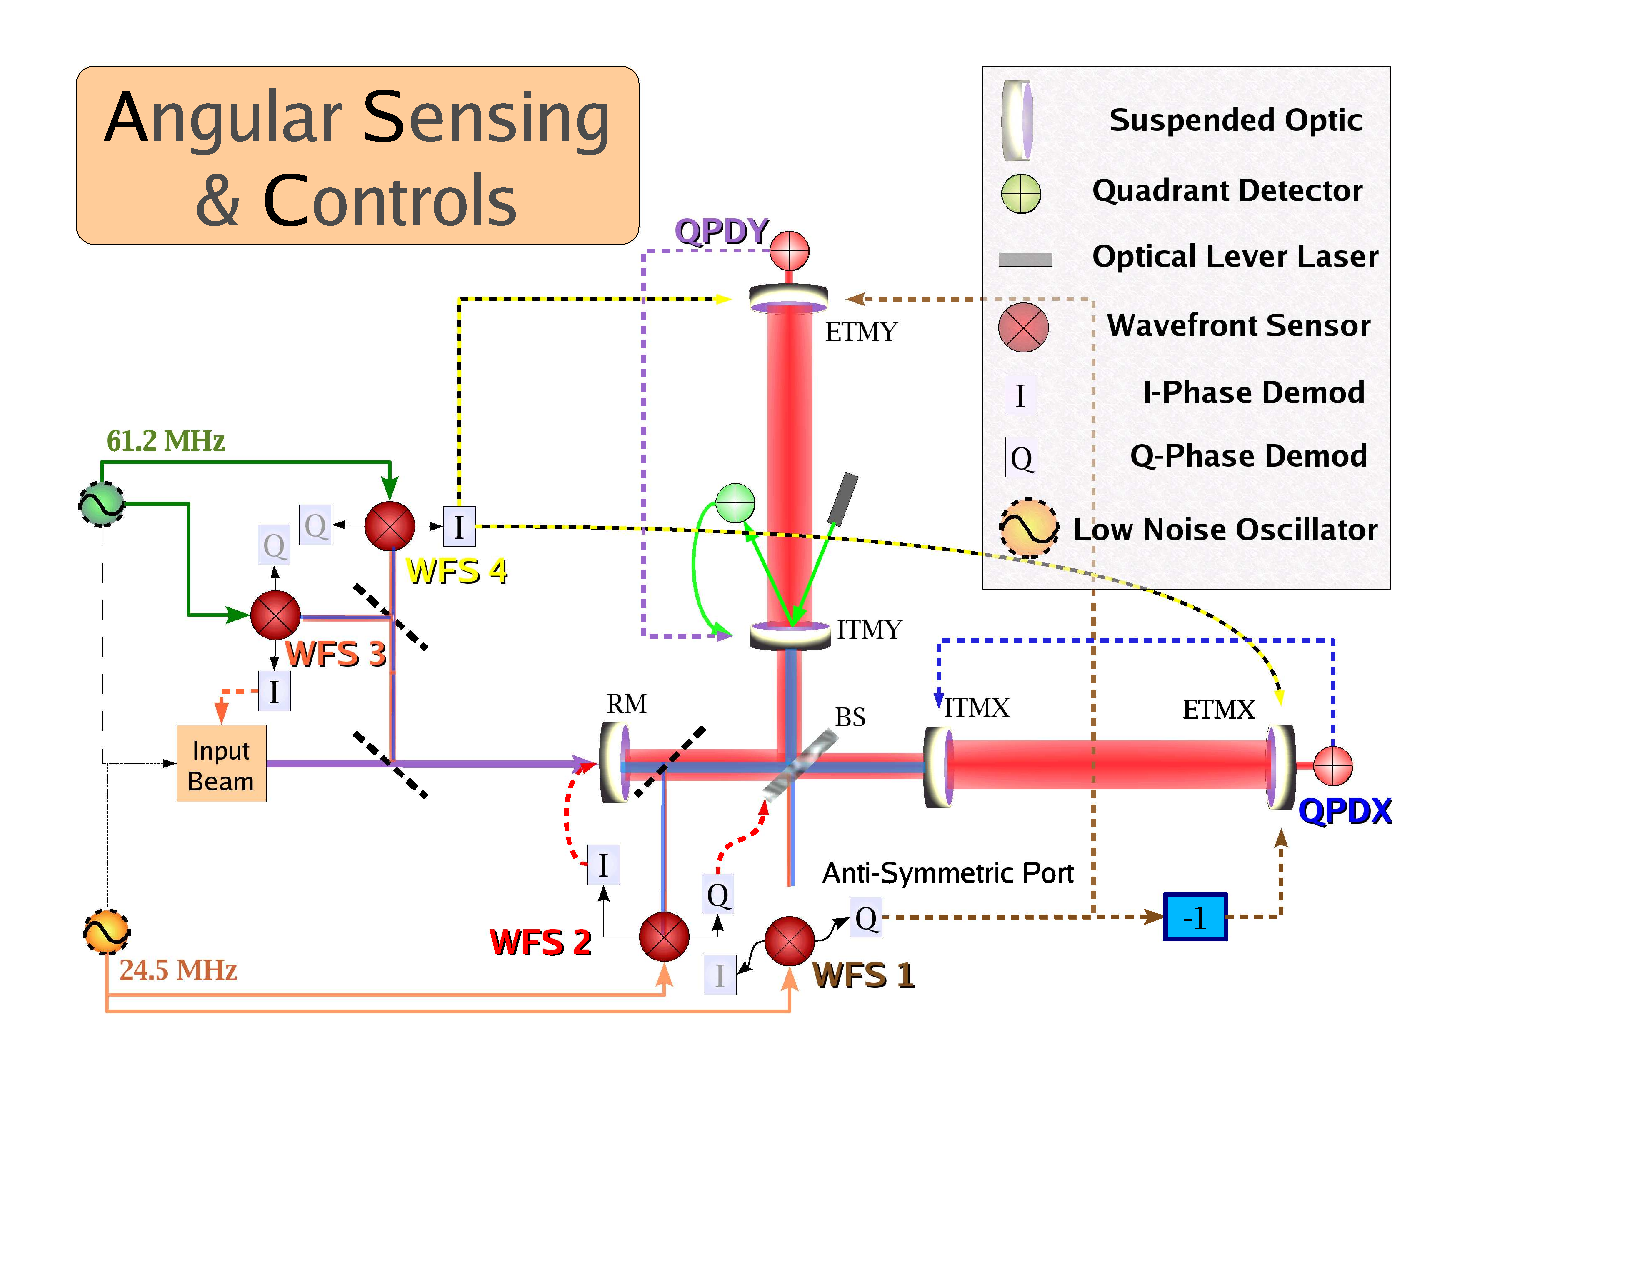
\includegraphics[angle=0,width=6.5in]{Figures/Chap5/ASC2.pdf}}
\caption[ASC Block Diagram]{Block diagram of the Angular Sensing and Control
                            system. Only one optical lever setup is shown for
                            simplicity, although there is one per optic.}
\label{fig:ASCblock}
\end{figure}

Figure~\ref{fig:ASCblock} shows a rough outline of the sensing and feedback
topology. Each of the suspended large optics has an optical lever servo. The
feedback diagram is a simplified version of the real feedback topology which
uses multiple mirrors in the feedback for each WFS. This arrows in this diagram
are only to indicate the principle degree of freedom of the feedback. 

During the S2 run, the Livingston interferometer had only WFS1 running,
with feedback set to drive the differential ETM angle. This is the most
critical angle in the interferometer; without control of this degree of
freedom, the power at the Anti-Symmetric port varies wildly, making many
servos unstable. The Hanford 4 km interferometer had nearly all of the 
WFS loops closed with a low bandwidth and for the S3 run managed to close all
WFS loops. 

\section{Local Damping}
\label{sec:OSEMs}

The wire suspension (see Section \ref{sec:SUS}) for the interferometer's central mirrors
is soft in 4 of 6 DOFs: The two vertical modes have
resonant frequencies from 10-20~Hz whereas, the horizontal eigenfrequencies are all from
0.5-1 Hz. To reduce the off-resonance thermal noise in the suspension wires,
the mechanical losses have been kept as low as possible. The result is that the
mechanical Q's are quite high; the intrinsic Q's of the suspended optic's free
body modes are estimated to be $\sim10^{5}$. Since the suspension structure
is actually perched on a lightly damped isolation stack, the Q's of the
full coupled resonant system are limited to $\sim10^{3}$.

This is still very large and so to prevent uncontrolled swinging of the optic,
it is locally damped by sensing its motion with respect to the suspension 
frame and feeding back with a force proportional to the velocity.

The sensors and actuators used for local control of the suspended optic
are described in Section~\ref{sec:OSEMdesc}.
The overview screen for the digital/analog
controls of one of the suspended test masses is shown in 
Figure~\ref{fig:SUSscreen} (this is also a good block diagram for how
the suspended optic is controlled).

\begin{figure}[!h]
\centerline{
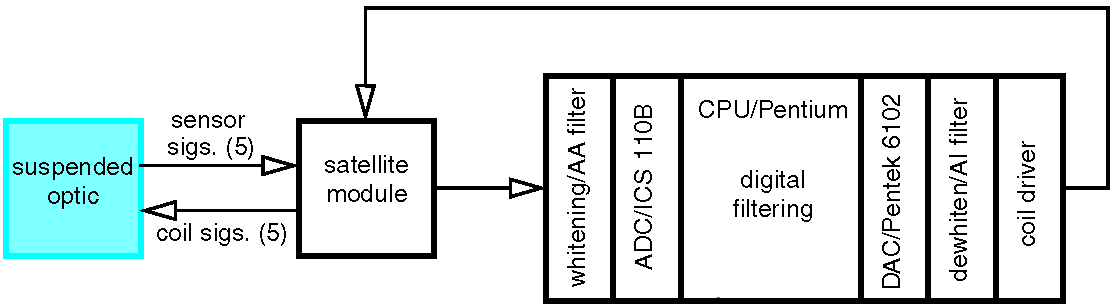
\includegraphics[angle=0,width=6.5in]{Figures/Chap5/LocalDamping.png}}
\caption[OSEM wiring]{Block diagram for the local damping electronics.}
\label{fig:SUSwiring}
\end{figure}

\begin{figure}[!h]
\centerline{
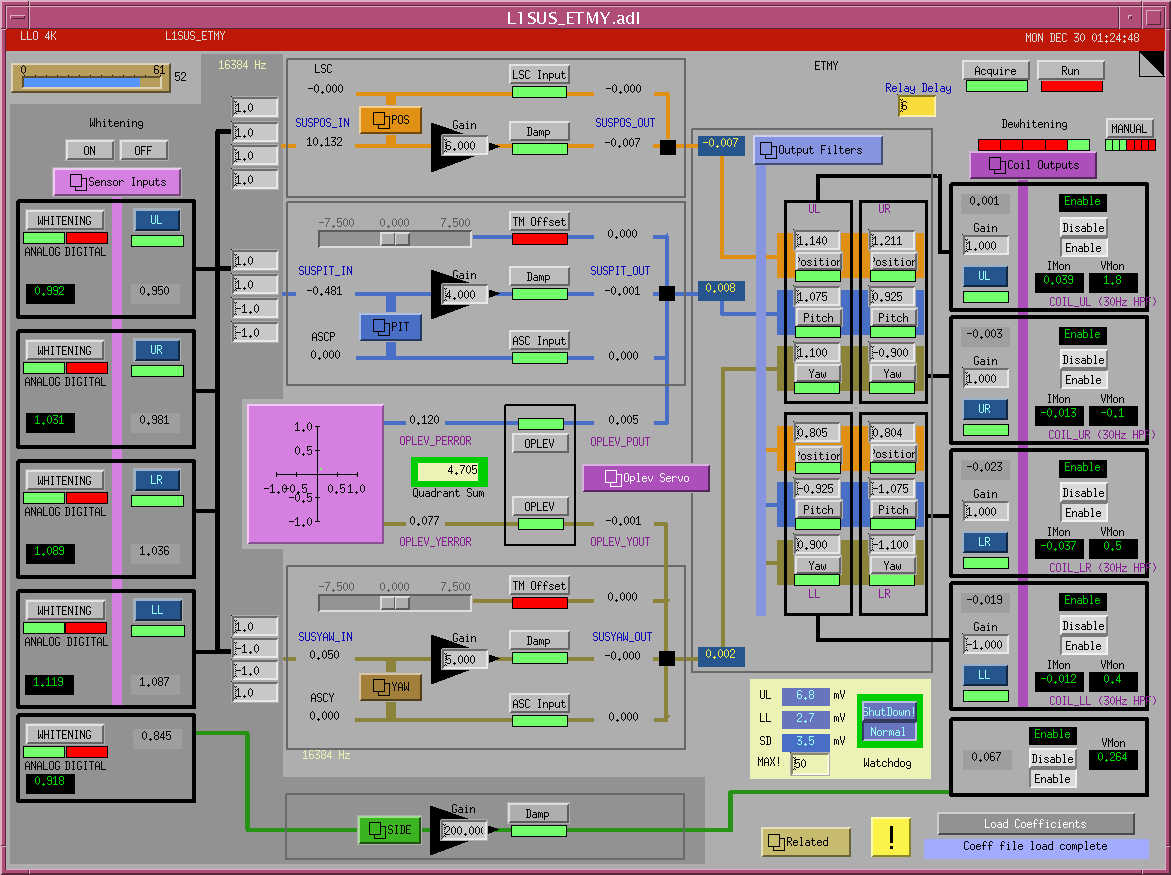
\includegraphics[angle=0,width=6.5in]{Figures/Chap5/L1SUS_ETMY.jpg}}
\caption[SUS Screen]{Overview screen for the ETMY digital suspension controls.}
\label{fig:SUSscreen}
\end{figure}

The signals from the 4 shadow sensors on the mirror face are conditioned,
acquired by an ADC, and then recombined in appropriate combinations to
reproduce signals corresponding to 3 of the free body modes of the optic.
Translation perpendicular to the optic face, pitch, and yaw are sensed
and then controlled. Vertical motion and rotation around the axis perpendicular
to the optic's face are not sensed or controlled. The sideways translation
of the optic is damped through the use of only one sensor/actuator pair.

The sensing noise of the shadow sensor 
is $\approx1 \times 10^{-10} \, \mbox{m}/\sqrt{\mbox{Hz}}$
above 20~Hz, limited mostly by shot noise in the detected light power. Since this
is 8 orders of magnitude above the displacement noise goal at 40 Hz, the filtering
must be aggressive enough to allow a gain of more than 1 for stable damping around 
1 Hz and also introduce less than 
$5 \times 10^{-19} \, \mbox{m}/\sqrt{\mbox{Hz}}$ of displacement noise at 40 Hz. 
Figure~\ref{fig:OSEMfilter} shows the open loop gain of the damping loop for
the piston degree of freedom.


\begin{figure}[!h]
\centerline{
\includegraphics[angle=0,width=6.5in]{Figures/Chap5/POSdamp.pdf}}
\caption[Pendulum Damping]{Magnitude of the open loop gain for the suspended
                           optic's piston degree of freedom.}
\label{fig:OSEMfilter}
\end{figure}




\section{Seismic Servos}
Seismic noise in the gravitational wave band affects the strain sensitivity directly by moving
the test masses. The largely unattenuated seismic disturbance below 20 Hz, 
however, is several orders of magnitude larger than the in-band noise. These 
low frequency motions impact the strain sensitivity non-linearly:

\begin{itemize}
 \item To keep the optical cavities resonant in the presence of large
   disturbances, the actuators must have a proportionally large dynamic
   range. Reducing the dynamic range with a fixed attenuator would proportionally
   reduce the noise contribution.

\item Due to the finite gain in the control servos the cavity lengths are pulled
   off of resonance, leading to bilinear up-conversion (see 
   Section~\ref{sec:residual_req} and Figures \ref{fig:POBnoise} 
   and \ref{fig:S1noiseComp} for examples).

\item There is a finite amount of light scattered at each optical surface. Some of
   this light is re-introduced into the signal readout path, producing a
   parasitic optical resonator around the main interferometer. In the regime
   where multiple wavelengths are traveled the scattered light noise can
   show up in the signal band.

\item Worst of all, often the ground noise is so large as to prevent any
   operation of the interferometer. At some point the velocities become so
   large that the lock acquisition system can no longer bring the optical
   cavities into resonance.
\end{itemize}


\subsubsection{Earth Tides}

The tidal gravitational forces from the moon and the sun distort the 
earth with a $\approx$12 hour period. These strains are
seasonally modulated, but on average create displacements of $\approx$400 
microns peak-peak over a 4 km baseline. This displacement exceeds 
the dynamic range of the test mass coil drivers ($\approx$ 10 microns).

To remove this large signal, the near DC component of the drive signals to the
end test masses' coil drivers are fed to higher dynamic range 
(180 microns peak-peak) actuators made of piezo-electric stacks. 
This system was designed to finely actuate the seismic isolation stack
at low frequencies. It is called the Fine Actuation System (FAS).

The strains from the earth tide can be divided into common and differential 
components. The common mode component can be accommodated by adjusting the 
laser wavelength as is done for the common mode servo. To accommodate 
a change, $\Delta L_{+}$, in the common mode arm length the laser 
frequency must shift by  
$\Delta \nu = \Delta L_{+} \frac{c/\lambda}{L_{arm}}$. 
This is $\simeq$7 MHz for a 100 micron length change. The slow, 
temperature actuator of the laser's master oscillator can easily give several 
hundred MHz of frequency shift.

Using an earth tide prediction program~\cite{Fred:Tides}, 
a large portion of the tidal strain was offloaded from the 
FAS in this manner on the Hanford interferometers. Figure~\ref{fig:TidalPred}
shows a comparison of the measured tidal strains with the predictions for the
Livingston interferometer during the S2 science run from February - April 2003.
From the small size of the residuals it looks like implementing the feed
forward to the laser wavelength would significantly reduce the size of the
feedback signals sent to the external seismic actuators and should be done
in the future.


\begin{figure}[!h]
\centerline{
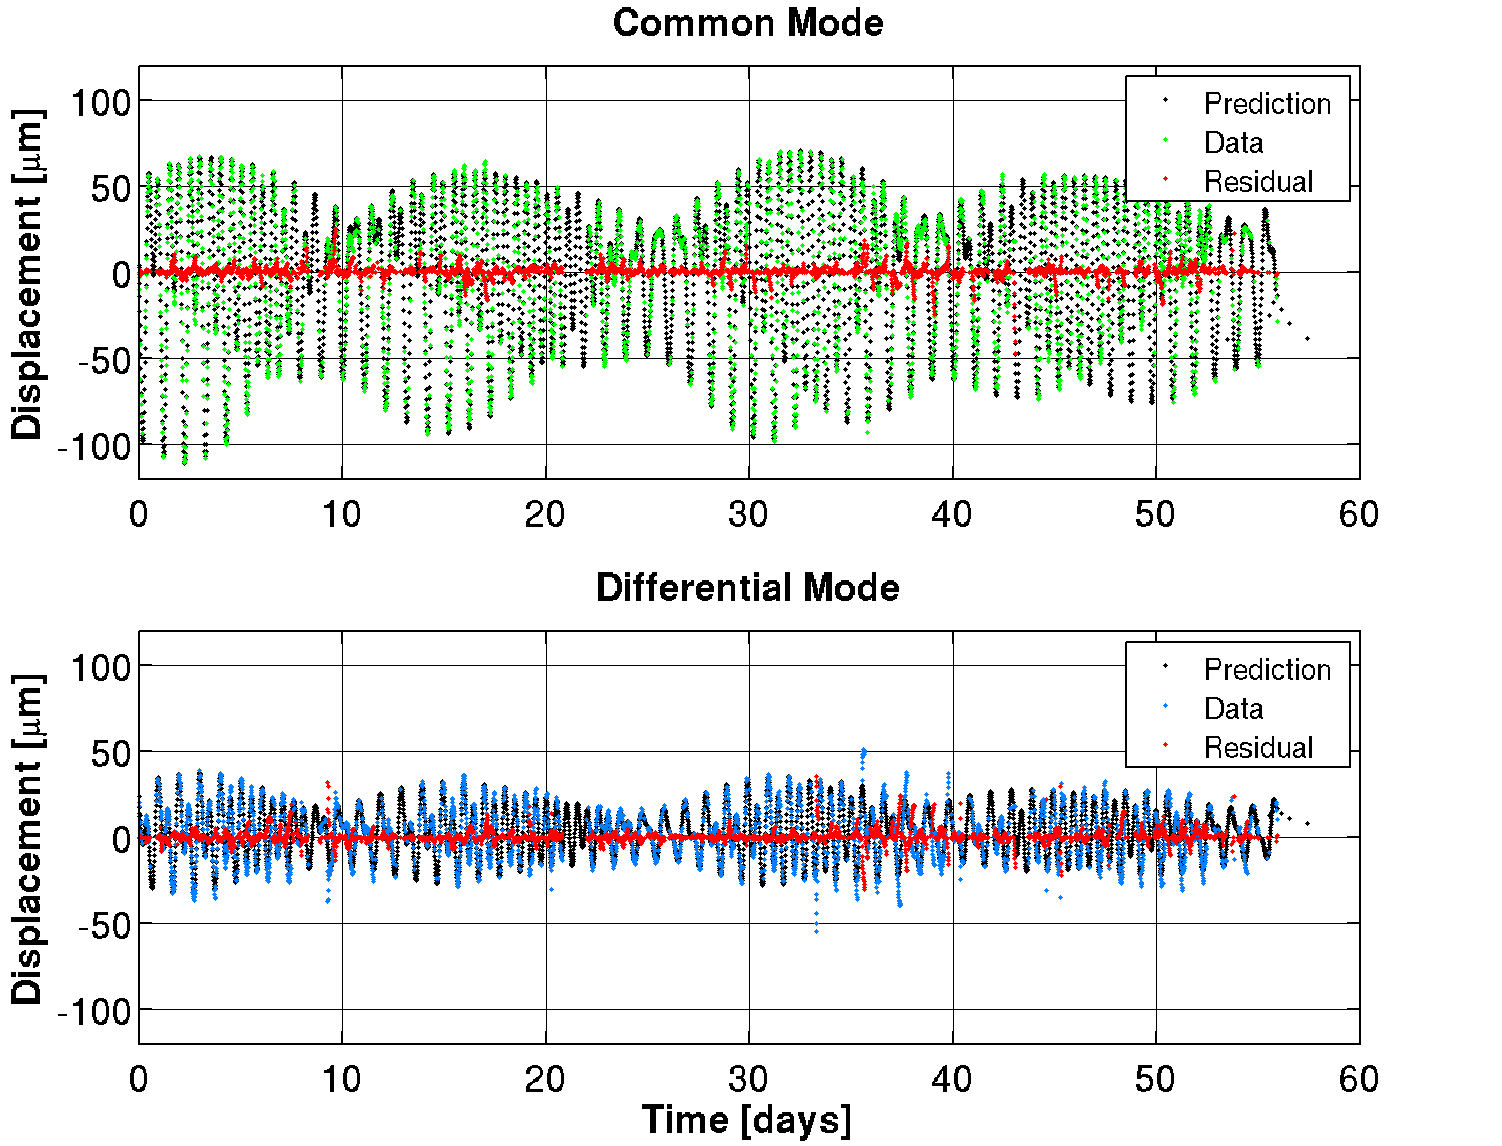
\includegraphics[angle=0,width=6.5in]{Figures/Chap5/Tides.png}}
\caption[Tidal Prediction]{The common and differential mode earth tide displacements
         are shown. Also plotted are the calibrated piezo control signals (the real
         displacements) and residual (data-prediction).}
\label{fig:TidalPred}
\end{figure}


\subsection{Microseismic Feed-Forward}

All over the earth, the largest ground motions (excepting earthquakes) are from the
$\sim$6 second period microseism discussed in Section~\ref{sec:SeismicCharacter}.

To reduce the arm length fluctuations from 0.1-0.5 Hz, a feed forward
scheme was implemented to measure the ground noise and apply this through
suitable filtering to the FAS~\cite{Giaime:MSFF}. An excellent, low frequency
seismometer (Streckheisen STS-2) was placed in each building to measure the
local microseismic motion. By measuring the displacement in each building
separately we were able to predict the microseismic arm length change and
send this signal into the second input of the FAS on the end test mass chambers 
to reduce the relative motions between the mirrors at the two ends of the arms.

Figure~\ref{fig:PEPI} shows an example of the effect of the feed forward on
the length fluctuations of a single arm cavity.

\subsection{Piezo-electric Pre-Isolator}

Out of necessity, the Livingston site was patched with 2 types of active
isolation to lower the influence of the ground motion.

As seen in Figure~\ref{fig:StackTF} the low frequency, high Q resonances of the
stack actually amplify the ground noise at some frequencies. This effect,
coupled with the large levels of anthropogenic noise, produce the large velocities
which impede interferometer operation. To reduce this effect, we installed a
local, Piezo-Electric Pre-Isolation (PEPI) system~\cite{Giaime:PEPI}.

PEPI works by sensing the sensing the horizontal velocities on the support
structure of the isolation stack and then using a stand alone computer with DSP
to feedback and reduce the seismic noise in the $\sim$0.5-3 Hz band. The
true power of PEPI comes from the digital nature of the feedback compensation.
The servo loop shape was tailored to exactly suppress the noise at the frequencies
where the isolation stack resonances would otherwise amplify. The PEPI feedback
goes into the third input of the FAS.

\begin{figure}[!h]
\centerline{
\includegraphics[angle=0,width=6.5in]{Figures/Chap5/PEPI-onoff.pdf}}
\caption[PEPI Performance]{Shows the differential arm length control signal
                   in units of velocity. The PEPI ON and PEPI OFF traces
                   show the reduction in the arm length velocities with
                   the PEPI servos on.}
\label{fig:PEPI}
\end{figure}



